\documentclass[letterpaper, 12pt]{article}

\usepackage{graphicx}
\usepackage{longtable}
\usepackage{rotating}
\usepackage{dcolumn}
\usepackage{listings}
\usepackage{subfiles}
\usepackage{amsmath}

% Code listing commands
\lstset{language=R,
basicstyle=\scriptsize\ttfamily,
commentstyle=\ttfamily,
numbers=left,
numberstyle=\footnotesize,
stepnumber=1,
numbersep=5pt,
showspaces=false,
showstringspaces=false,
showtabs=false,
frame=single,
tabsize=2,
captionpos=b,
breaklines=true,
breakatwhitespace=false,
title=\lstname,
escapeinside={},
keywordstyle={},
morekeywords={}
}

\begin{document}
\title{ARE213 Problem Set \#2A}
\author{Peter Alstone \& Frank Proulx}
\maketitle

\section{Problem \#1 and \#2}
These are hand written and attached separately.
%\subsection{Part A}
%Here we will consider the within estimator, as suggested. This suggests that we want to find $\widehat{\beta_{FE}}$ by running the following regression:
%\begin{equation}
%\ddot{Y_{it}} = \ddot{X'_{it}}\widehat{\beta_{FE}} + \ddot{\epsilon_{it}}
%\end{equation}
%Where $\ddot{Y_{it}}=Y_{it}-\bar{Y_i}$, $\ddot{X_{it}}=X_{it}-\bar{X_i}$, $\bar{Y_i}=\frac{1}{T}\sum_{t=1}^TY_{it}$, and $\bar{X_i}=\frac{1}{T}\sum_{t=1}^TX_{it}$.
%Our fixed effects estimator is therefore
%
%\begin{equation}
%\widehat{\beta_{FE}}=(\ddot{X'_{it}}\ddot{X_{it}})^{-1}\ddot{X'_{it}}\ddot{Y_{it}} %His notes say you ``don't have to invert the mega-matrix'', so I might be doing this wrong.
%\end{equation}
%
%Because we have T=2, this can be rewritten as
%\begin{equation}
%\widehat{\beta_{FE}}=((X_{it}-\frac{1}{2}X_{i1}-\frac{1}{2}X_{i2})'(X_{it}-\frac{1}{2}X_{i1}-\frac{1}{2}X_{i2}))^{-1}(X_{it}-\frac{1}{2}X_{i1}-\frac{1}{2}X_{i2})'(Y_{it}-\frac{1}{2}Y_{i1}-\frac{1}{2}Y_{i2})
%\end{equation}
%
%
%
%
%And looking at the first differences estimator, where we get $\widehat{\beta_{FD}}$ by running the regression
%\begin{equation}
%\Delta Y_{it} = \Delta X'_{it} \widehat{\beta_{FD}} + \Delta \epsilon_{it}
%\end{equation}
%
%where $\Delta Y_{it} = Y_{it} - Y_{it-1}$, $\Delta X_{it} = X_{it} - X_{it-1}$, and $\Delta \epsilon_{it} = \epsilon_{it} - \epsilon_{it-1}$.
%
%Because we only have T=2, this differencing estimator can only be estimated for t=2, so we regress
%\begin{align}
%\Delta Y_{i2} = \Delta X'_{i2} \widehat{\beta_{FD}} + \Delta \epsilon_{i2} \\
%Y_{i2}-Y_{i1} = (X_{i2}-X_{i1})'\widehat{\beta_{FD}} + \epsilon_{i2}-\epsilon_{i1}
%\end{align}
%
%thus, our first difference estimator is
%\begin{equation}
%\widehat{\beta_{FD}}=((X_{i2}-X_{i1})'(X_{i2}-X_{i1}))^{-1} (X_{i2}-X_{i1})'(Y_{i2}-Y_{i1})
%\end{equation}

\section{Problem \#3}
\subsection{Part A}
Running pooled bivariate OLS, adding a quadratic time trend, and adding the covariates that we expect to belong produces the models shown in Table \ref{tab:3a}.  The pooled OLS is an ill-informed baseline model but nonetheless tells us that there is a statistically significant negative correlation between the states with primary seatbelt laws and those without.  In particular, the mean of the log fatalities per capita is reduced by 0.14 for states with primary seatbelt laws.  This does not, however, account for the year to year trends that are captured by including a set of quadratic year terms in the regression as shown in the ``quadratic time" regression.  This basic trend is that deaths have gone down over time.  Correcting for these trends may allow our OLS estimates approach the true ATE, and indeed the apparent effect of primary seatbelt laws is reduced.  When further covariates are added that are relevant (see Table \ref{tab:3a}) further reductions in the apparent effect occur and the effect is no longer statistically significant.  
\subfile{p3a.tex}

\begin{figure}[htbp]
\begin{center}
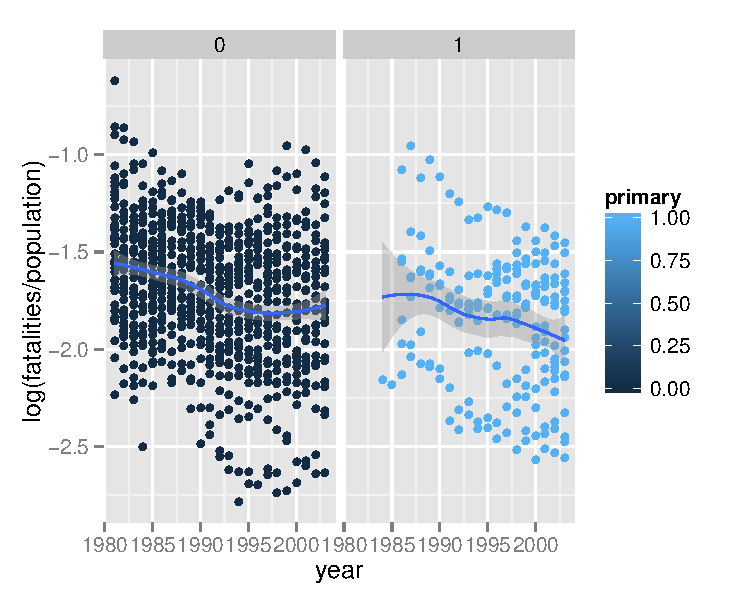
\includegraphics{plot3a.pdf}
\caption{Year to year trends in the log of traffic fatalities per capita, divided by primary seatbelt law presence.  A LOESS fit to each dataset is included for reference but is not necessarily indicative of the true underlying function.}
\label{fig:3a}
\end{center}
\end{figure}



\subsection{Part B}
No, the standard errors are most likely not correct (are they ever really, truly correct outside a purely theoretical framework?).  In this case the error in the SE estimates comes from heteroscedasticity in the error terms from the regression.  Table \ref{tab:3b1} shows that introducing robust standard errors (using the HC1 estimator for the OLS covariance matrix).  Clustering on the state grouping only increases the SE slightly over the robust pooled version, indicating most of the heteroscedasticity is in the full sample and not within-group.  
Table \ref{tab:3b2} shows the results of calculating the standard errors by hand, using the code shown in the code listings section at the end (with a call out to that section of code).

\subfile{p3b1.tex}
\subfile{p3b2.tex}


\subsection{Part C}
The between estimator will give an unbiased estimate of the effect of primary seat belt laws insofar as variation within states (across time) is uncorrelated with the observables.
\subfile{p3c.tex}

We don't think that this criterion is met here. For example, within a given state, the total vmt per year probably tracks very closely with fatalities, as the higher VMT within a given year, the more likely there are to be fatal crashes (ceteris paribus).  

%% I don't know what to say about standard errors. -- my best shot at it below...still hazy.
The standard errors are sufficiently large in this model that we cannot rule out the null hypothesis (no effect of primary seatbelt laws) in either the simple case or the case with covariates. 

\subsection{Part D}
The RE estimator will give an unbiased estimate so long as the within states variation is uncorrelated with observables. Again, this assumption is probably not met here.  In the RE model we find (for the first time) that seat belt laws appear to be correlated with statistical significance with reduced fatalities....but do we trust these?  Table \ref{tab:p3d} summarizes the results for the RE model both with and without covariates.  
\subfile{p3d.tex}

The Random Effects estimator has the advantage over pooled OLS that it allows for (and assumes) unobserved heterogeneity. OLS has the advantage that it is more efficient than the Random Effects estimator when said heterogeneity does not exist.

\subsection{Part E}

The conventional standard errors for the RE model are likely incorrect because of a built-in assumption that the errors within each individual are correlated equally over time.  Because this is a long-term dataset we would prefer to relax this assumption by introducing robust clustered SE estimates.  Table \ref{tab:p3e} shows that this increases the SE of the coefficient on primary seatbelt use, but only by about double.  The SE is still small compared to the estimand.

\subfile{p3e.tex}

\subsection{Part F}

The conventional and clustered standard errors differ (as they have for many other approaches) by about a factor of two in the FE method.  These are compared in Table \ref{tab:p3f}.  The baseline standard errors (or roughly the coefficient of variation) is small for the fixed effects model because all of the unobserved individual state characteristics are wrapped up in the FE model without any between-ness muddying their influence.  However, there remain heteroscedastic errors within each state from idiosyncrasies  between time periods when states did and did not have seat belt laws (national-level trends, automobile manufacturing standards, etc.) that are exogenous to the states and link them.  Figure \ref{fig:3f} shows how the adoption of state-level primary seatbelt laws occurred non-uniformly through the sample.
% this is my best attempt at this...

\subfile{p3f.tex}

\begin{figure}[htbp]
\begin{center}
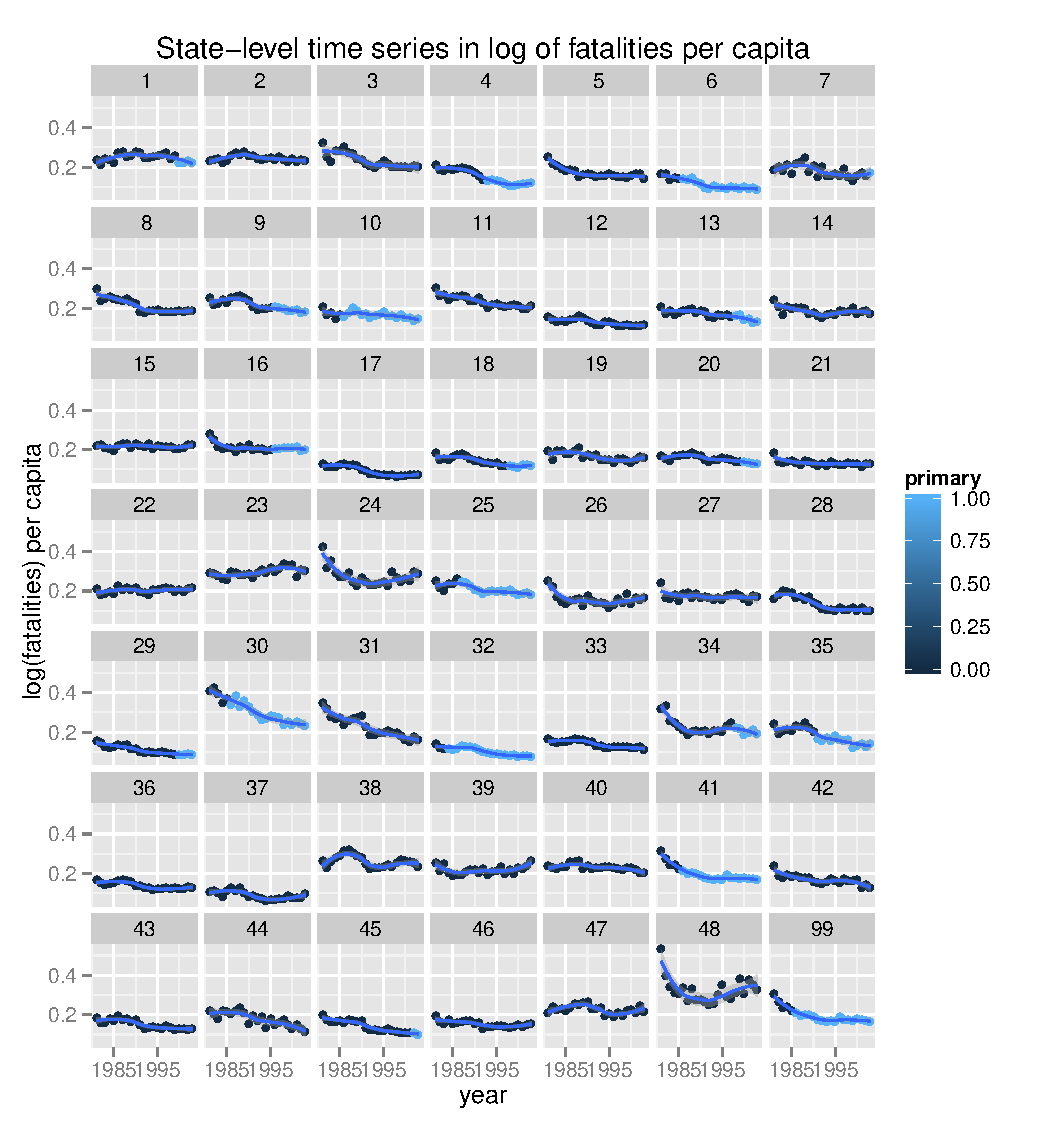
\includegraphics{allstates.pdf}
\caption{Year to year trends in the log of traffic fatalities per capita, with facets by state ID.  A LOESS fit to each dataset is included for reference but is not necessarily indicative of the true underlying function.}
\label{fig:3f}
\end{center}
\end{figure}


\subsection{Part G}

The addition of covariate terms to the FE model reduces the estimate of the ATE for enacting primary seatbelt laws to about a 6\% reduction in annual fatalities.  With robust / clustered standard errors this is estimate maintains its significance at a 5\% confidence level. 

\subfile{p3g.tex}

\section{Code Listings}

We used R to complete this assignment...which turned out to be quite challenging in this case, since R has no equivalently easy version of ``robust" or ``cluster(group)," but it was a learning experience.  The code is below:

\lstinputlisting{ps2a-paworking.R}


\subsection{Hand-coded HC Robust Clustered Standard Errors}

\begin{lstlisting}
## Robust by hand
#This calculates the Huber-White Robust standard errors -- code based on http://thetarzan.wordpress.com/2011/05/28/heteroskedasticity-robust-and-clustered-standard-errors-in-r/
s <- summary(pooled.full)
X <- model.matrix(pooled.full)
u2 <- residuals(pooled.full)^2
XDX <- 0

for(i in 1:nrow(X)) {
    XDX <- XDX +u2[i]*X[i,]%*%t(X[i,])
}

# inverse(X'X)
XX1 <- solve(t(X)%*%X)

#Compute variance/covariance matrix
varcovar <- XX1 %*% XDX %*% XX1

# Degrees of freedom adjustment
dfc <- sqrt(nrow(X))/sqrt(nrow(X)-ncol(X))

stdh <- dfc*sqrt(diag(varcovar))

t <- pooled.full$coefficients/stdh
p <- 2*pnorm(-abs(t))
results.robust <- cbind(pooled.full$coefficients, stdh, t, p)
dimnames(results.robust) <- dimnames(s$coefficients)
results.robust

## cluster by hand -- using many of the same variables as defined in the robust section (above), with some modifications:
cluster <- "state"
clus <- cbind(X, "state"=ps2a.data[,cluster], "resid" = resid(pooled.full))
                                        #number of clusters
m <- dim(table(clus[,cluster]))
k <- dim(X)[2]

uj <- matrix(NA, nrow=m, ncol = k)
gs <- names(table(ps2a.data[,cluster]))
for (i in 1:m){
    uj[i,] <- t(matrix(clus[clus[,cluster]==gs[i], 'resid'])) %*% clus[clus[,cluster]==gs[i], 1:k]
}


#Compute variance/covariance matrix
varcovar <- XX1 %*% crossprod(uj) %*% XX1

# Degrees of freedom adjustment
dfc <- sqrt((m/(m-1)) * (nrow(X)-1)/(nrow(X)-ncol(X)))

stdh <- dfc*sqrt(diag(varcovar))

t <- pooled.full$coefficients/stdh
p <- 2*pnorm(-abs(t))
results.cluster <- cbind(pooled.full$coefficients, stdh, t, p)
dimnames(results.cluster) <- dimnames(s$coefficients)
results.cluster

hand.comparison <- cbind(a.typ.full[,2], results.robust[,2], results.cluster[,2])
colnames(hand.comparison) <- c("Conventional", "Robust", "Clustered")
stargazer(data.frame(hand.comparison),
          summary = FALSE,
          title = "Comparison of Standard Error HC Methods for Full Pooled Model, as calculated by hand",
          style = "qje",
          out = 'p3b2.tex',
          font.size = "footnotesize", 
          column.labels = c("Conventional", "HC1 Robust", "HC1 Robust + Cluster"),
          label="tab:3b2"
          )
\end{lstlisting}

\lstinputlisting{../util/are213-func.R}

\end{document}
